\documentclass[12pt]{article}
\usepackage{amsmath}
\usepackage{amssymb}
\usepackage{amsthm}
\usepackage{mathtools}
\usepackage{hyperref}
\usepackage{graphicx}
\usepackage{enumerate}
\usepackage[utf8]{inputenc}
\usepackage[english]{babel}
\newcommand{\R}{\mathbb{R}}

\newtheorem*{theorem}{Theorem}
\newtheorem*{corollary}{Corollary}
\newtheorem*{proposition}{Proposition}
\newtheorem*{lemma}{Lemma}


\title{Algorithmic Operation Research \\ From Linear to Conic Duality}
\date{14-1-2020}
\author{Theodora Panagea - 1115201400135 \\ Anna-Aikaterini Kavvada - 1115201500050}


\begin{document}
\begin{figure}
    \centering
    
\includegraphics[width=10cm]{nkua.png}
    
\end{figure}
       
\begin{figure}

    \centering
    
\includegraphics[width=8cm]{dit.png}
\end{figure}

\maketitle{}
\begin{center}
\instructor{Professor: Anna Karasoulou}

\end{center}
  	\pagenumbering{arabic}
  	\newpage
  	\tableofcontents
  	\newpage
  	
\section{Introduction}  	
  	 Linear Programming (LP) models cover numerous applications. Whenever applicable, LP allows to obtain useful quantitative and qualitative information on the problem at hand. The specific analytic structure of LP programs gives rise to a number of general results, which provide us in many cases with valuable insight and understanding. This analytic structure underlies some specific computational techniques for LP, which by now are perfectly well developed, allowing us to solve routinely quite large LP programs. However, there are situations in reality which cannot be covered by the LP models. To handle these "essentially nonlinear" cases, one needs to extend the basic theoretical result and computational techniques known for LP beyond the bounds of Linear Programming.\\
  	The widest class of optimization problems to which the basic results of LP were extended, is the class of convex optimization problems. Below, follows a definition of a general convex optimization problem. This definition is not the traditional, but it suits well to the applications we intend to cover.\\ 
  	When passing from a generic LP problem 
  	$$\max\limits_{x} \{ c^T x | Ax \geq b \} \quad [A: m \times n] \quad (LP)$$
  	to its nonlinear extensions, we should expect to encounter some nonlinear components in the
    problem. The traditional way here is to say that in (LP), there are a linear objective function $f(x) = c^T x$ and inequality constraints $f_i (x) \geq b_i$ with linear functions $f_i (x) = a_i^T x,\quad i = 1, ..., m$. Let us allow some/all of these functions $f, f_1 , ..., f_ m$ to be nonlinear. In contrast to this traditional way, we intend to keep the objective and the constraints linear, but introduce “non-linearity” in the inequality sign $\geq$.
    \subsection{Definitions}
    
   The constraint inequality $Ax \geq b$ in (LP) is an inequality between vectors; as such, it requires a definition: given two vectors a, b $\in \R^m$, we write $a \geq b$, if the coordinates of $a$ majorate the corresponding coordinates of b:
   \begin{align*}
   a \geq b \Leftrightarrow \{ a_i \geq b_i. \quad i = 1, \ldots, m \} \quad (\geq)
   \end{align*} \newpage
    The above “coordinate-wise” partial ordering of vectors in $\R^m$ satisfies a number of basic properties of the standard ordering of reals; namely, for all vectors $a, b, c, d, ... \in \R^m$ one has:
    \begin{enumerate}
    		\item \textit{Reflexivity:} $a \geq a$
    		\item \textit{Anti-Symmetry:} if both $a \geq b$ and $b \geq a$, then $a = b$
    		\item \textit{Transitivity:} if both $ a\geq b$ and $b \geq c$, then $a \geq c$
    		\item \textit{Compatibility with linear operations:}
    			\begin{itemize}
    				\item \textit{Homogeneity:} if $a \geq b$ and $\lambda$ is a nonnegative real, then $\lambda a \geq \lambda b$ \\ ("One can multiply both sides of an inequality by a nonnegative real")
				\item \textit{Additivity:} if both $a \geq b$ and $c \geq d$, then $a + c \geq b + d$ \\ ("One can add two inequalities of the same sign")
    			\end{itemize}
    \end{enumerate}
   Thus, we observe that
    \begin{itemize}
	\item A significant part of the nice features of LP programs comes from the fact that the vector inequality $\geq$ in the constraint of (LP) satisfies the properties 1. – 4.;
	\item The standard inequality  ” $\geq$ ” is neither the only possible, nor the only interesting way to define the notion of a vector inequality fitting the axioms 1. – 4.
\end{itemize}
Therefore, we can conclude to the following: 
\paragraph*{A generic optimization problem which looks exactly the same as (LP), up to the fact that the inequality $\geq$ in (LP) is now replaced with and ordering which differs from the component-wise one, inherits a significant part of the properties of (LP) problems. Specifying properly the ordering of vectors, one can obtain from (LP) generic optimization problems covering many important applications which cannot be treated by the standard (LP). \newpage} 

We have to define the "geometry" of a "vector inequality", bearing in mind the  axioms 1. – 4. Consequently, we pick vectors from a finite-dimensional Euclidean space $E$ with an inner product $ \langle \cdot, \cdot \rangle$ and reach the assumption that $E$ has a partial ordering (called also vector inequality), let's refer to it as $\succeq:$. In other words, we define the pairs of vectors $a, b$ from $E$ linked by the inequality $a \succeq b$. We call the ordering “good”, if it obeys the axioms 1. – 4., and will examine what these good orderings are. \\  \\
At first, we observe that: \\ 
\textit{A good vector inequality $\succeq$ is completely identified by the set \emph{K} of $\succeq$-nonnegative vectors:}
$$K = \{ a \in E: a \succeq 0 \}$$ 
\textit{Furthermore,}
$$ a \succeq b \Leftrightarrow a - b \succeq 0 \quad [\Leftrightarrow a - b \in K]$$
Let's prove the above statement. Let $a \succeq b$. By 1. we have $-b \succeq -b$, and by 4.(b) we may add the two inequalities with the same sign, to get $a - b \succeq 0$. If $a - b \succeq 0$, then, adding to this inequality the $b \succeq b$, we get $a \succeq b$. \\
It is clear that the set K cannot be arbitrary. It must satisfy the following conditions:
\begin{enumerate}
\item $K$ is nonempty and closed under addtion: $$a,a' \in K \Rightarrow a+a' \in K$$
\item $K$ is a conic set: $$a \in K, \lambda  \geq 0 \Rightarrow \lambda a \in K$$
\item $K$ is pointed: $$ a \in K \text{ and } -a \in K \Rightarrow a = 0$$
\end{enumerate} \newpage 
Therefore, it is easy to verify that $K$ is a pointed cone and geometrically, $K$ does not contain any straight lines passing through the origin.
\begin{figure}[h!]
	\begin{center}
  		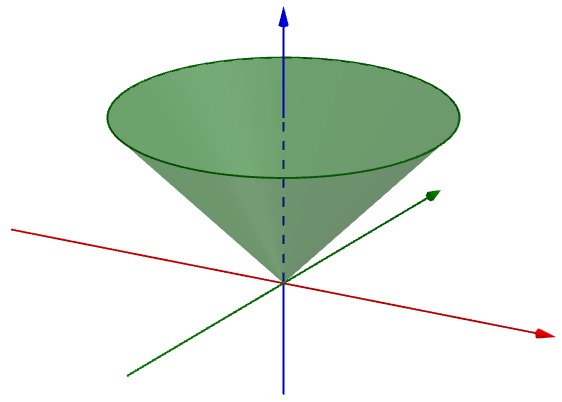
\includegraphics[width=7cm]{pointed_cone.png}
  		\caption{A pointed cone}
	  \end{center}
\end{figure}
\\
	Hence, every pointed cone $K$ in $E$ leads to a partial ordering on $E$, satisfying the axioms 1.-4. We symbolize this ordering with $\geq_{\kappa}$:
	$$a \geq_{\kappa} b \Leftrightarrow a - b \geq_{\kappa} 0 \Leftrightarrow a- b \in K$$
The cone comprised of vectors with nonnegative entries (the nonnegative orthant) is the one responsible for the standard coordinate-wise ordering $\geq$ on $E = \R^m$:
$$ \R^{m}_{+} = \{ x = (x_1, \ldots, x_m)^T \in \R^m: x_i \geq 0, i = 1, \ldots, m \}$$
We are going to use the standard shorthand notation $a \geq b$, instead of $a \geq_{\R^{m}_{+}}  b$ \\
The nonnegative orthant $\R^{m}_{+}$ is not just a pointed cone, but it also possesses the following properties:
\begin{flushright}
\begin{enumerate}[I.]
\item The cone is closed: if a sequence of vectors $a_i$ from the cone has a limit, the latter also belongs to the cone.
\item The cone possesses a nonempty interior: there exists a vector such that a ball of positive radius centered at the vector is contained in the cone.
\end{enumerate}  
\end{flushright}

\paragraph{From now on, speaking about vector inequalities $\geq_{\kappa}$, we always assume that the underlying set $K$ is a pointed and closed cone with a nonempty interior. \newline}

Note that the closedness of $K$ makes it possible to pass to limits in $\geq_{\kappa}$-inequalities: $$a_i \geq_{\kappa} b_i,\quad a^i \rightarrow a, b^i \rightarrow b \text{ as } i \rightarrow \infty \Rightarrow a \geq_{\kappa} b $$.
The nonemptiness of the interior of K allows to define, along with the “non-strict” inequality a $a \geq_{\kappa} b$ , also the strict inequality according to the rule 
$$ a > _\kappa b \Leftrightarrow a-b \in \text{ int} K$$
where int$K$ is the interior of the cone $K$. \\ \\
\textbf{Examples:} Some interesting cones with partial orderings, are the following: 
\begin{itemize}
\item The nonnegative orthant $\R^m_{+}$ in $\R^n$
\item The Lorentz (or the second-order, or the less scientific name the ice-cream) cone
$$L^m =\Bigg\{ \quad  x = (x_1, \ldots, x_{m-1}, x_m)^T \in \R^m : x_m \geq \sqrt{\sum^{m-1}_{i =1}x^2_i} \quad \Bigg\}$$
\item The semidefinite cone $S_+^m$. This cone is in the space $E = S^m$ of $m\times m$ symmetric matrices (equiped with the Frobenius inner product $\langle A, B \rangle =$ Tr$(A,B) = \sum_{ij}A_{ij}B_{ij}$) and consists of all $m \times m$ matrices $A$ which are positive semidefinite, i.e.,
$$A = A^T; \quad x^T Ax \geq 0 \quad \forall x \in \R^m $$

\end{itemize}
    \newpage
    \section{What is Conic Duality?}
    Apart from the algorithmic issues, the most important result in LP is the LP Duality Theorem. This theorem, can be extended further to cover convex and conic problems, the latter being a subcategory of the former. \par
    The source of the LP Duality Theorem was the desire to get in a systematic way a lower bound on the
    optimal value $c^*$ in an LP program
    $$c^* = \min\limits_{x} \{ c^T x | Ax \geq b \}. \quad (LP)$$
    The bound was obtained by looking at the inequalities of the type 
    $$\langle \lambda, Ax\rangle \equiv \lambda^T Ax \geq \lambda^T b \quad (Cons(\lambda))$$
    with weight vectors $\lambda \geq 0$. This type of inequality is, by its origins, a consequence of the system of constraints $Ax \geq b$ of LP, i.e., it is satisfied at every solution to the system. As a consequence, whenever we are lucky to get, as the left hand side of $(Cons(\lambda))$, the expression $c^T x$, i.e., whenever a nonnegative weight vector $\lambda$ satisfies the relation 
    $$A^T \lambda = c,$$
    then, the inequality $(Cons(\lambda))$ produces a lower bound $b^T \lambda$ on the optimal value in LP 
    and the dual problem 
    $$max \{b^T \lambda : \lambda \geq 0, A^T \lambda = c\}$$
    was nothing but the problem of finding the best lower bound one can get in this way.\par
    Coming to think of a conic problem, the same strategy can be used to develop its dual
    $$\min \{ c^T x | Ax \geq_{\kappa}b \}, \quad K \subset E \quad (CP)$$ \newpage
    At this point, we need to clarify the following step: \\ \\
    \textit{What are the “admissible” weight vectors $\lambda$, i.e., the vectors such that the scalar 
    inequality}
    $$\langle \lambda, Ax\rangle \geq \langle \lambda, b\rangle$$
    \textit{is a consequence of the vector inequality} $Ax \geq_{\kappa} b ?$ \\ \\
    In the particular case of coordinate-wise partial ordering, i.e., in the case of $E = R^m , K = R_+^m $, 
    the admissible vectors were those with nonnegative coordinates. These vectors, however, not necessarily 
    are admissible for an ordering $\geq \kappa$ when $K$ is different from the nonnegative orthant. \\ 
    \subsection{The Dual Cone}
    In order to define Conic Duality, we need to introduce the dual cone ($K_*$) and its properties. \\
 	The set $K_*$ is comprised of vectors whose inner products with all vectors from $K$ are nonnegative. $K_*$ is called the cone dual to $K$. \\
 	\begin{theorem}[Properties of the dual cone] Let $E$ be a finite-dimensional Euclidean space with inner product $\langle \cdot, \cdot \rangle$ and let $K \subset E$ be a nonempty set. Then
 		\begin{enumerate}[(i)]
			\item The set $$K_* = \{ \lambda \in E^m \langle \lambda , a \rangle \geq 0 \quad \forall a \in K \}$$is a closed cone 		
 			\item If int$K \neq \emptyset $, then $K_*$ is pointed.
 			\item If $K$ is a closed convex pointed cone, then int $K_* \neq \emptyset$.
 			\item If $K$ is a closed cone, then so is $K_*$, and the cone dual to $K_*$ is $K$ itself:
 			$$(K_*)_* = K$$
 		\end{enumerate}
 	\end{theorem} 
 	An immediate corollary of the Theorem is as follows:
 	\begin{corollary}
 	 A set $K \subset E$ is a regular (i.e., closed, convex, pointed and with a nonempty interior) cone if and only if the set $K_*$ is so.
 	\end{corollary} \newpage
 	\subsection{The Dual Problem of a Conic Problem}
 	Following the above, as in the case of (LP), we observe, as an immediate consequence of the definition of $K_*$, that whenever $x$ is a feasible solution to conic primal problem (P) and $\lambda$ is an admissible weight vector, i.e., $\lambda \in K_*$, then $x$ satisfies the scalar inequality:
 	$$(A^* \lambda)^T x \equiv \langle \lambda, Ax \rangle \geq \langle \lambda, b \rangle $$
 	Thus, whenever $\lambda_*$ is an admissible weight vector satisfying the relation $$A^*\lambda = c $$
 	we have 
 	$$c^Tx = (A^*\lambda)^T x = \langle \lambda, Ax \rangle \geq \langle b, \lambda \rangle $$
 	for all $x$ feasible for (P), so that $\langle b, \lambda \rangle$ is a lower bound on the optimal value of (P). The best bound is the optimal value in the problem:
 	$$max\{ \langle b, \lambda \rangle: A^* \lambda = c, \lambda \geq_{\kappa_*} 0  \}$$
 	and this program is called the dual program (D) to (P). 
 	To conclude, we have reached to the following proposition, which we will analyse further, at the next section.
 	\begin{proposition}
 	[Weak Conic Duality Theorem] The optimal value of (D) is a lower bound on the optimal value of (P).
 	\end{proposition}
 	
   \section{Conic Duality Theorem}
    For this section, let us call the following program as the conic primal, and name it (CP):
    \begin{align*}
 \text{Maximize } \quad  &\langle c,x \rangle \\
\text{subject to } \quad  &b - Ax \in L &
\tag{P}\\
 &x \in K   			
   	\end{align*}
   	Then, we define its dual (CD) as the conic program below:
   	 \begin{align*}
\text{Minimize } \quad  &\langle b,y \rangle \\
\text{subject to } \quad  &A^Ty - c \in K^* &
\tag{D}\\
  &y \in L^*   			
   	\end{align*}
   	In linear programming, we assume that one of the two programs, let's say (LD) is feasible. Firstly we prove the \textit{weak duality}: If the primal program (LP) is subfeasible, the subvalue of (LP) is upper-bounded by the value of (LD). The weak duality has the important consequence that (LD) - a minimization problem - has finite value if (LP) is subfeasible. \\
   	Then we prove \textit{regular duality:} there is no gap between the subvalue of (LP) and the. \\
   	Similarly, we have to prove the following, in order to establish the conic duality: \\
   	1. Symmetry \\ 
	2. Weak Conic Duality Theorem \\
	3. Strong Conic Duality Theorem \\

	\subsection{Symmetry}
   	Let's change the (D), in order to have the same format as the (CP).
   	\begin{align*}
    \text{Maximize } \quad  -&\langle b,y \rangle \\
     \text{subject to } \quad  -&c + A^Ty \in K_* 
     \tag{D}
     \\
 	&y \in L^*   			
   	\end{align*}
	Having done this, we can easily compute the dual of (D') which leads us back to (P). Now, we can continue with the Weak and Strong Duality.   \\First, we prove \textit{weak duality:} If the primal program (P) is subfeasible, the subvalue of (P) is upper-bounded by the value of (D). Weak duality has the important consequence that (D)—a minimization problem—has finite value if (P) is subfeasible. \\
	Then we prove \textit{regular duality:} there is in fact no gap between the subvalue of (P) and the value of (D). There was no need for that in LP, but here the following scenario is possible: both (P) and (D) are feasible, but there is a gap between their values $\gamma$ and $\beta$.
	\begin{figure}[ht]
	\begin{center}
  		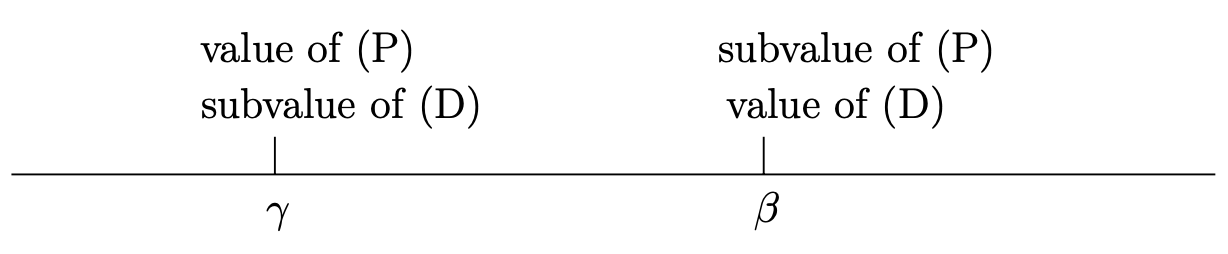
\includegraphics[width=10cm]{fig2.png}
  		\caption{Gap between the values of (P) and (D) cone program}
	  \end{center}
\end{figure} \newpage
In order to get \textit{strong duality}, we apply Slater’s constraint qualification: If one of the programs has an interior point, then the other program is feasible as well, and there is no gap between their values.	
    
    \subsection{Weak Conic Duality Theorem}
    \begin{theorem}
    If the dual program $(D)$ is feasible, and if the primal program
$(P)$ is subfeasible, then the subvalue of $(P)$ is upper-bounded by the value of $(D)$.
\end{theorem}
If $(P)$ is feasible as well, this implies that the value of $(P)$ is upper-bounded by the value of $(D)$, and that both values are finite. This is weak duality as we know it from linear programming.
\begin{proof}
     We pick any feasible solution $y$ of $(D)$ and any feasible sequences $(x_k)_{k \in \mathbb{N}}$, $(x'_k)_{k \in \mathbb{N}}$ of (P). Then we know that
     $$ 0 \leq \langle \underbrace{A^T y - c}_{\in  K_*}, \underbrace{x_k}_{\in K} \rangle + \langle \underbrace{y}_{\in L_*}, \underbrace{x'_k}_{\in L} \rangle = \langle y, Ax_k + x'_k \rangle - \langle c, x_k \rangle, k \in \mathbb{N} $$
     Hence, 
     $$\limsup_{k\rightarrow \infty}{\langle c, x_k \rangle} \leq \limsup_{k\rightarrow \infty}{\langle y, Ax_k + x'_k \rangle} = \langle c, b \rangle $$
     Since the feasible sequences were arbitrary, this means that the subvalue of $(P)$ is upper-bounded by $\langle y, b \rangle$, and since $y$ was an arbitrary feasible solution of $(D)$, the lemma follows.
     
\end{proof}
    \subsection{Regular Conic Duality Theorem}
    Here is the Regular duality theorem. The proof essentially consists of applications of the Farkas Lemma, to carefully crafted systems. \\
    \begin{lemma}
    [Farkas Lemma] Let $K \subseteq V$ be a closed convex cone, and $b \in W$. The system $Ax = b, x \in K$ is subfeasible if and only if every $y \in W$ with $A^Ty \in K_*$ also satisfies $\langle y, b \rangle \geq 0$
    \end{lemma}
    
    \begin{theorem}
    The dual program $(D)$ is feasible and has finite value $\beta$ if and only if the primal program $(P)$ is subfeasible and has finite subvalue $\gamma$. Moreover, $\beta = \gamma$.
    \end{theorem}
    \begin{proof}
         If $(D)$ is feasible and has value $\beta$, we know that
         \begin{align*}
            A^Ty - c \in K_*, y \in L_* \quad  \Rightarrow  \quad \langle b,y \rangle \geq \beta 
            \tag{I}
         \end{align*}
         We also know that
         \begin{align*}
             A^Ty \in K_*, y \in L_* \quad \Rightarrow \quad  \langle b,y \rangle \geq 0
             \tag{II}
         \end{align*}
         
    Indeed, if we had some $y$ that fails to satisfy the latter implication, we could add a large positive multiple of it to any feasible solution of $(D)$ and in this way obtain a feasible solution of value smaller than $\beta$.
    Merging the(I) and (II), we get: 
    \begin{align*}
        A^Ty - zc \in K_*, y\in L_*, z \geq 0 \rightarrow \langle \beta, y \rangle \geq z \beta.
        \tag{III}
    \end{align*}
    For $z > 0$, we obtain this from (I) by multiplication of all terms with $z$ and then renaming $zy \in L_*$ back to $y$. For $z = 0$, it is simply (II). In matrix form, we can rewrite (III) as follows: 
    \begin{align*}
    \Bigg(
    \begin{tabular}{c|c}
        $A^T & -c$ \\
        \hline
        id & 0 \\
        \hline 
        0 & 1 
        \end{tabular} \Bigg) (y,z) \in K_* \oplus L_* \oplus R_+ \quad \Rightarrow \quad (b^T|− \beta)(y,z) \geq 0 
        \tag{IV}
        \end{align*}
    Here and in the following, we use a column vector $c \in V$ as the linear operator z $\mapsto$ zc from $\R$ to $V$ and the row vector $c^T$ as the (adjoint) linear operator $x \mapsto \langle c, x \rangle$ from $V$ to $\R$. The form (IV) now allows us to apply the Farkas lemma. The implication (IV) holds if and only if
    \begin{align*}
    \Bigg(
    \begin{tabular}{c|c|c}
        A & id & 0 \\
        \hline
        $-c^T & 0^T & 1$ \\
    \end{tabular} \Bigg) (x, x', z) = (b, -\beta), (x, x', z) \in  (K_* \oplus L_* \oplus R_+)_* = K \oplus L \oplus R_+ 
        \tag{V}
    \end{align*}
    is subfeasible. 
    The above system is subfeasible if and only if there are sequences
           $ (x_k)_{k \in \mathbb{N}}, (x′_k)_{k\in \mathbb{N}}, (z_k)_{k \in \mathbb{N}}$ with $x_k \in K, x'_k \in L, z_k \geq 0$ for all $k$, such that
           \begin{align*}
               \lim_{k \rightarrow \infty} Ax_k + x'_k = b
               \tag{VI} \\
            \end{align*}
            and
            \begin{align*}
               \lim_{k \rightarrow \infty} \langle c, x_k \rangle - z_k = \beta 
              \tag{VII}
           \end{align*}
Now (VI) shows that (P) is subfeasible, and (VII) shows that the subvalue of (P) is at least $\beta$. Weak duality shows that it is at most $\beta$, concluding the “only if” direction. \\
For the “if” direction, let (P) be subfeasible with finite subvalue $\gamma$ and assume for the purpose of obtaining a contradiction that $(D)$ is infeasible. This yields the implication
\begin{align*}
    A^T y - zc \in K_*, y \in L_*, \rightarrow z \leq 0 
    \tag{VIII}
\end{align*}
since for any pair $(y,z)$ that violates it, $\frac{1}{z}y$ would be a feasible solution of (D).
We now play the same game as before and write this in Farkas-lemma-compatible matrix form:
\begin{align*}
    \Bigg(
    \begin{tabular}{c|c}
        $A^T & -c$ \\
        \hline
        id & 0 \\
    \end{tabular} \Bigg)
    (y, z)\in K_* \oplus L_* \Rightarrow (0^T|-1)(y,z) \geq 0
    \tag{IX}
\end{align*}
That means that the system 
\begin{align*}
    \Bigg(
    \begin{tabular}{c|c}
        $A & id$ \\
        \hline
        -c^T & 0 \\
    \end{tabular} \Bigg)
    (x, x') = (0,-1), (x,x') \in K \oplus L
    \tag{X}
\end{align*}
is subfeasible, which in turn means that there are sequences $(x_k)_{k \in \mathbb{N}}, (x'_k)_{k \in \mathbb{N}}$ with $x_k \in K$, $x'_k \in L$ for all k, such that
\begin{align*}
    \lim_{k\rightarrow \infty} Ax_k + x'_k = 0 
    \tag{XI} \\
    \lim_{k\rightarrow \infty} \langle c, x_k \rangle = 1 
    \tag{XII}
\end{align*}
But this is a contradiction: Elementwise addition of $(x_k)_{k \in \mathbb{N}},(x'_k)_{k \in \mathbb{N}}$ to any feasible sequences of (P) that witness subvalue $\gamma$ would result in feasible sequences that yield subvalue at least $\gamma + 1.$ \\
Consequently, the dual program (D) must have been feasible. Weak duality yields that (D) has finite value $\beta  \geq \gamma$. But then $\beta = \gamma$ follows from the previous “only if” direction.
    \end{proof} 
    
    \subsection{Strong Conic Duality Theorem}
  Here is the \textbf{strong Duality Theorem of Cone Programming}, under Slater’s
constraint qualification.
\begin{theorem}
If the primal program (P) is feasible, has finite value γ and has
an interior point $\tilde{x}̃$, then the dual program (D) is feasible and has finite value $\beta = \gamma$.
\end{theorem}

\begin{proof}
(P) is in particular subfeasible, and since the program has an interior
point, that means that the subvalue of (P) is also $\gamma$. Using the regular Duality Theorem (“if” direction), the statement follows.
\end{proof}

The strong Duality Theorem is not applicable if the primal cone program
(P) is in equational form $(L = \{0\})$, since the cone $L = \{0\}$ has no interior points.
But there is a different variant of Slater’s constraint qualification that we can use in this case, given that $V$, $W$ are finite-dimensional.

\begin{theorem}
    Assume that the Hilbert spaces V and W are finite- dimensional. If the primal program
    \begin{align*}
 \text{Maximize } \quad  &\langle c,x \rangle \\
\text{subject to } \quad  &Ax = b &
\tag{P}\\
 &x \in K   			
   	\end{align*}
is feasible, has finite value $\gamma$ and has a point $\tilde{x} \in \mathrm{int} (K)$ such that $A \tilde{x} = b$, then the dual problem 
 \begin{align*}
 \text{Minimize } \quad  &\langle b,y \rangle 
 \tag{D}
 \\
\text{subject to } \quad  &A^Ty - c \in K_* 
   	\end{align*}
   	is feasible and has finite value $\beta = \gamma$.
\end{theorem}
We remark that for general $L$, just requiring a point $\tilde{x} \in \mathrm{int}(K)$ with $b - A \tilde{x} \in L$. is not enough to achieve strong duality. 
    
    \section{Geometry of Primal and Dual Problems}
    Let's consider the geometry of primal (P) and dual (D) conic problems:
    
    $$ \min \{c^Tx|Ax \geq_\kappa b \} \text{\hspace{2.3cm}} (P) $$
    $$ \max \{\langle b, \lambda \rangle | A^*\lambda = c, \lambda \geq_{\kappa^*} 0 \} \quad (D) $$
    where we can observe that their in-between structure looks quite different and this difference is due to data representation. However, we will examine them more carefully, and prove that geometrically, the problems (P) and (D) are completely similar. 
    \subsection{From Algebra to Geometry}
    In (D) our main goal is to maximize a linear objective $\langle b, \lambda \rangle$, over the intersection of an affine plane $L_* = \{ \lambda : A^* \lambda = c \}$ with the cone $K_*$. \\
    In (P), if $x$ are "true design variables", we get their images $y = Ax - b \in E$. When $x$ runs through $\R_n$, $y$ runs through the affine plane $L = \{y = Ax - b : x \in \R_n\}$; $x \in \R_n$ is feasible for (P) if and only if the corresponding $y = Ax - b$ belongs to the cone $K$. \\
    So, in (P) we have the intersection of the affine plane $L$ and the cone $K$, same fashion as (D).
     Having the image of $x$ $y = Ax - b$, we can express the objective $c^Tx$ it as follows: 
     \begin{align}
     c^Tx = \langle d, Ax - b \rangle + \text{const} \equiv c \in \text{Im}{A^*}
     \end{align}
     where (P) can be expressed as: $$\min\limits_{y}\{ \langle d,y \rangle : y \in L, y \geq_{\kappa} 0 \}$$
     since $L = \text{Im}A - b$, $A^*d = c$ and $d$ is any vector satisfying the above relation. 
     \paragraph{The primal problem (P) (1), geometrically, is the problem of minimizing a linear form over the intersection of the affine plane $L$ with the cone $K$. The dual problem (D), similarly, is to maximize another linear form over the intersection of the affine plane $L_{\**}$ with the dual cone $K_{\**}$. \\ \\}
     However, if the conditions for (P) are not met, the problem is eather unbounded below, or infeasible. Thus, we reject (P) from the very beginning. Therefore, we assume that (1) is satisfied. \\
     \subsection{Relation between (P) and (D) Problems}
     To wrap this up, we need to explain the relation between the geometric data of (P) and (D) problems. Now we are aware of the association of cone $K_*$ being the dual cone of $K$, in (D) and (P) problems respectively. Following that, we also know that the feasible $L$ and $L_*$ are orthogonal to each other ($L_* \perp L$). More specifically, $L$ is the translation by vector -b, of the linear subspace 
     $$\mathcal{L} = \text{Im}A \equiv \{ y = Ax : x \in \R^n \} $$
     In the same fashion, we get the linear subspace $\mathcal{L_*}$ of the dual,  which is derived from the translation of $L_*$ with any solution $\lambda_0$ of $A^*\lambda = c$.
     $$\mathcal{L_*} = \mathrm{Null}(A^*) \equiv \{ \lambda : A^* \lambda = 0
     \}$$
     From Linear Algebra we know that $\mathcal{L}$ and $\mathcal{L_*}$ are also orthogonal complements of each other. \\
     We reach the following geometrical conclusion, as far as the conic problem is concerned: 
     \begin{align*}
     \min\limits_{y}\{ \langle d,y \rangle : y \in \mathcal{L}-b, y \geq_{\kappa} 0 \}
     \tag{P}
     \end{align*}
     where (P) is a problem of minimizing a linear objective $\langle d, y \rangle$ over the intersection of a cone $K$ with an affine plane $L = \mathcal{L} - b$ given as a translation, by vector $-b$, of a linear subspace $\mathcal{L}$. \\ \\
     Its dual problem is: 
     \begin{align*}
     \max\limits_{\lambda}\{ \langle b,\lambda \rangle : \lambda \in \mathcal{L}^{\perp}+d , \lambda \geq_{\kappa_*} 0 \}
     \tag{D}
     \end{align*}
     where (D) is a problem of maximizing the linear objective $\langle b, \lambda \rangle$ over the intersection of the dual cone $K_*$ with an affine plane $L_* = \mathcal{L}^{\perp}+d$ given as a translation, by the vector d, of the orthogonal complement $\mathcal{L}^\perp$ of $\mathcal{L}$. \newpage
     From Weak Conic Duality, we know that $(K_*)_* = K$ and $(\mathcal{L}^\perp)^\perp = \mathcal{L}$. The geometry and the above symmetry of (P) and (D) is illustrated below: 
     \begin{figure}[ht]
	\begin{center}
  		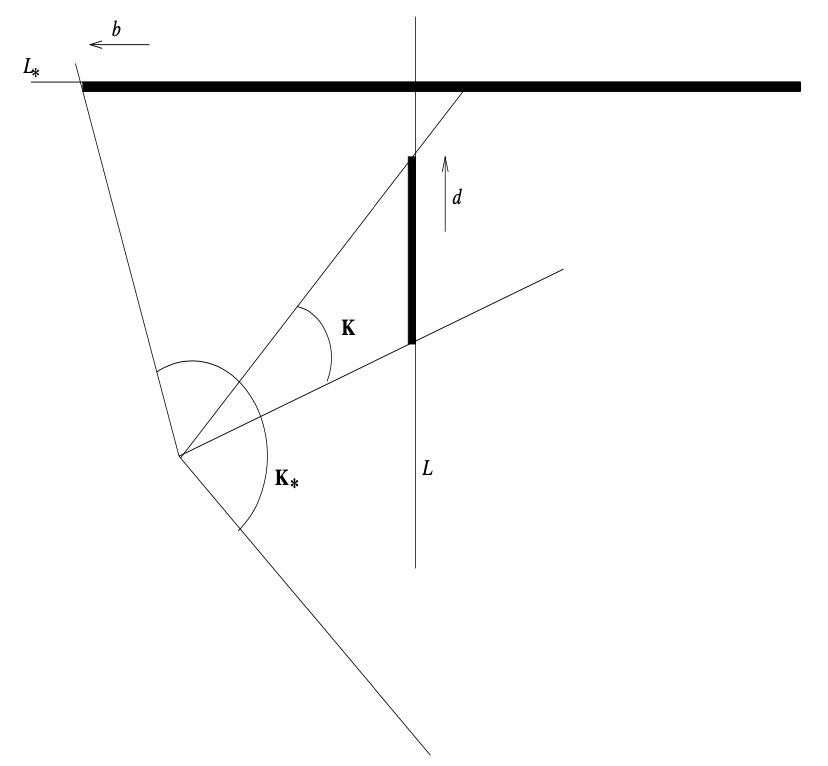
\includegraphics[width=9cm]{fig1.png}
  		\caption{Primal-dual pair of conic problems \newline [bold: primal (vertical segment) and dual (horizontal ray) feasible sets]}
	  \end{center}
\end{figure}
    
    \section{Applications of Conic Duality }
    
    \subsection{Self-Dual Cones}
    The cone $K_*$ is the dual of the cone $K$, and if $K_* = K$, then the cone is called \textbf{self-dual}. Some self-dual cones are the following: 
    
    \begin{itemize}
    \item The nonnegative orthant $\R^m_{+}$ in $\R^n$
    \item The Lorentz (or the second-order, or the less scientific name the ice-cream) cone
    $$L^m =\Bigg\{ \quad  x = (x_1, \ldots, x_{m-1}, x_m)^T \in \R^m : x_m \geq \sqrt{\sum^{m-1}_{i =1}x^2_i} \quad \Bigg\}$$
    \item The semidefinite cone $S_+^m$. This cone is in the space $E = S^m$ of $m\times m$ symmetric matrices (equiped with the Frobenius inner product $\langle A, B \rangle =$ Tr$(A,B) = \sum_{ij}A_{ij}B_{ij}$) and consists of all $m \times m$ matrices $A$ which are positive semidefinite, i.e.,
    $$A = A^T; \quad x^T Ax \geq 0 \quad \forall x \in \R^m $$
    \end{itemize}
    \subsection{Second Order Cone Programming (SOCP)}
    In a second-order cone program (SOCP) a linear function is minimized over the intersection of an affine set and the product of second-order (quadratic) cones. SOCPs are nonlinear convex problems that include linear and (convex) quadratic programs as special cases, and arise in many engineering problems, such as filter design, antenna array weight design, truss design, robust estimation, and problems involving friction (e.g., robot grasp).
    \subsection{Semidefinite Programming (SDP)}
    Semidefinite programming (SDP) is a subfield of convex optimization concerned with the optimization of a linear objective function over the intersection of the cone of positive semidefinite matrices with an affine space, i.e., a spectrahedron. \\ \\
Semidefinite programming is a relatively new field of optimization which is of growing interest for several reasons. Many practical problems in operations research and combinatorial optimization can be modeled or approximated as semidefinite programming problems. In automatic control theory, SDPs are used in the context of linear matrix inequalities. SDPs are in fact a special case of cone programming and can be efficiently solved by interior point methods. All linear programs can be expressed as SDPs, and via hierarchies of SDPs the solutions of polynomial optimization problems can be approximated. Semidefinite programming has been used in the optimization of complex systems. In recent years, some quantum query complexity problems have been formulated in terms of semidefinite programs. \newpage
    \subsection{Distributionally Robust Learning (DRL)}
    Distributionally Robust Learning (DRL) is necessary for building reliable machine learning systems. When machine learning is deployed in the real world, its performance can be significantly degraded because test data may follow a different distribution from training data. DRL explicitly considers the worst-case distribution shift by minimizing the adversarially reweighted training loss. 
    
   \section{Is Something Wrong?}
   The issue at hand, is that the Conic Duality Theorem is much weaker than the Linear Duality Theorem. In LP, feasibility (even non-strict) and boundedness of either primal or dual problem, implies solvability of both the primal and the dual and equality between their optimal values. In CP, if one of (P) and (D) is essentially stricly feasible and bounded, then the other is solvable with their optimal values are equal. If both are essentially strictly feasible, then both are solvable and their optimal values are equal. As a result, it is clear that, a “word-by-word” extension of the LP Duality Theorem to the conic case is false.

   \section{Consequences}
   \subsection{Sufficient Condition for Infeasibility}
   Recall that a necessary and sufficient condition for infeasibility of a (finite) system of scalar linear inequalities (i.e., for a vector inequality with respect to the partial ordering $\geq$) is the possibility to combine these inequalities in a linear fashion in such a way that the resulting scalar linear inequality is contradictory. In the case of cone-generated vector inequalities a slightly weaker result can be obtained: \newpage
   \begin{proposition}
   [Conic Theorem on Alternative] Consider a linear vector inequality:
   \begin{align*}
       Ax - b \geq_\kappa 0 
       \tag{I}
   \end{align*}
   \begin{enumerate}[i.]
   \item If there exists $\lambda$ satisfying 
   \begin{align*}
       \lambda \geq_{\kappa_{*}} 0, A^* \lambda = 0, \langle \lambda, b \rangle > 0
       \tag{II}
   \end{align*} 
   then (I) has no solutions.
   \item If (II) has no solutions, then (I) is "almost solvable"- for every positive $\epsilon$ there exists $b'$ such that $||b' - b||_2 < \epsilon$ and the perturbed system
   $$Ax - b' \geq_\kappa 0$$ is solvable. 
   \item (II) is solvable iff (I) is not "almost solvable".
   \end{enumerate}
   \end{proposition}
   
   \subsection{The Linear Inequality between a Scalar and a Linear Vector}
   We have the following linear vector inequality:
   \begin{align*}
       Ax \geq_\kappa b
       \tag{V}
   \end{align*}
   and a scalar inequality:
   \begin{align*}
       c^Tx \geq d
       \tag{S}
   \end{align*}
   we want to check whether (S) is a consequence of (V). In the case of $K$ being a nonnegative orthant, the answer is trivial, by the inhomogeneous Farkas Lemma:
   \paragraph{The linear inequality of scalar $(S)$ is a consequence of a feasible system of linear inequalities $Ax \geq b$ \textit{iff} $(S)$ can be obtained from linear vector $(V)$ and the trivial $1 \geq 0$ \\}
   \begin{proposition}
   \begin{enumerate}[(i)]
   \item If $(S)$ can be obtained from $(V)$ and from the trivial inequality $1 \geq 0$ by
admissible aggregation, i.e., there exist weight vector  $\lambda \geq_{\kappa_*} 0$ such that
 $$A^* \lambda = c,\langle \lambda,b \rangle \geq d$$ then $(S)$ is a consequence of $(V)$.
 \item If $(S)$ is a consequence of a strictly feasible linear vector inequality $(V)$, then $(S)$ can be obtained from $(V)$ by an admissible aggregation.
   \end{enumerate}
   \end{proposition}
   Note that the difference between the case of the partial ordering $\geq$ and a general partial ordering $\geq_\kappa$ is in the word “strictly” in (ii).
   \subsection{Robustness}
   In the general conic case we may meet “pathologies” which do not occur in LP. E.g., a feasible and bounded problem may be unsolvable, the dual to a solvable conic problem may be infeasible, etc. Where the pathologies come from? Looking at our “pathological examples”, we arrive at the following guess: the source of the pathologies is that in these examples, the “solvability status” of the primal problem is non-robust – it can be changed by small perturbations of the data. This issue of robustness is very important in modelling. \\
   A question of primary importance is whether the properties of the program (CP) (feasibility, solvability, etc.) are stable with respect to perturbations of the data. The reasons which make this question important are the following:
   \begin{itemize}
       \item In actual applications, especially those arising in Engineering, the data are normally inexact: their true values, even when they “exist in the nature”, are not known exactly when the problem is processed. Consequently, the results of the processing say something definite about the “true” problem only if these results are robust with respect to small data perturbations i.e., the properties of (CP) we have discovered are shared not only by the particular (“nominal”) problem we were processing, but also by all problems with nearby data.
       \item Even when the exact data are available, we should take into account that processing them computationally we unavoidably add “noise” like rounding errors. As a result, a real-life computational routine can recognize only those properties of the input problem which are stable with respect to small perturbations of the data. 
   \end{itemize}
   Due to the above reasons, we should study not only whether a given problem (CP) is feasi- ble/bounded/solvable, etc., but also whether these properties are robust – remain unchanged under small data perturbations. As it turns out, the Conic Duality Theorem allows to recognize “robust feasibility/boundedness/solvability...”. \\ \\
   In order to define Robust Feasibility, we have to introduce the following relevant concepts of (CP):
   \begin{itemize}
       \item robust feasible, if all “sufficiently close” problems (i.e., those of the same structure
(n, m, K) and with data close enough to those of (CP)) are feasible
\item robust infeasible, if all sufficiently close problems are infeasible
\item robust bounded below, if all sufficiently close problems are bounded below (i.e., their objectives are bounded below on their feasible sets)
\item robust unbounded, if all sufficiently close problems are not bounded
\item robust solvable, if all sufficiently close problems are solvable
   \end{itemize}
   \begin{proposition}
   [Robust Feasibility] $(CP)$ is robust feasible if and only if it is strictly feasible, in which case the dual problem $(D)$ is robust bounded above.
   \end{proposition}
   \begin{proposition}
   [Robust Infeasibility] $(CP)$ is robust infeasible if and only if the system 
   $$\langle b,\lambda \rangle = 1, A^* \lambda = 0, \lambda \geq_{\kappa_*} 0$$
   is robust feasible, or, which is the same (by Robust feasibility), if and only if the system
   $$\langle b,\lambda \rangle = 1, A^* \lambda = 0, \lambda \geq_{\kappa_*} 0$$ has a solution.
   \end{proposition}
    \newpage
   \begin{proposition}
   [Robust Solvability] For a conic problem $(CP)$ the following conditions are equivalent to each other:
   \begin{enumerate}[(i)]
   \item $(CP)$ is robust feasible and robust bounded (below)
   \item $(CP)$ is robust solvable
   \item $(D)$ is robust solvable
   \item $(D)$ is robust feasible and robust bounded (above)
   \item Both $(CP)$ and $(D)$  are strictly feasible
   \end{enumerate}
   In particular, under every one of these equivalent assumptions, both $(P)$ and $(D)$ are solvable with equal optimal values.
   \end{proposition}
   \newpage
   \section{Bibliography}
$[1]$ Ben-Tal, A. and Nemirovskiĭ, A. Lectures on Modern Convex Optimization. pp.52-71. (2013). \\ \\
$[2]$ O.Guler. Foundations of Optimization. Graduate Texts in Mathematics. Springer New York, (2010). \\ \\
$[3]$ David Williamson. Orie6300: Mathematical programming I, lecture 26. \href{http://people.orie.cornell.edu/dpw/orie6300/Lectures/
lec26.pdf}{http://people.orie.cornell.edu/dpw/orie6300/Lectures/
lec26.pdf}. \\ \\
$[4]$ B. Gartner and Matousek J. Approximation algorithms and semidefinite programming: Cone programming. \\ \\ \href{http://www.ti.inf.ethz.ch/ew/lehre/ApproxSDP09/notes/conelp.pdf}{http://www.ti.inf.ethz.ch/ew/lehre/ApproxSDP09/notes/conelp.pdf} \\ \\
$[5]$ Weihua Hu et. al, Does Distributionally Robust Supervised Learning Give Robust Classifiers? (2018) arXiv:1611.02041v6 \\ \\
$[6]$ Yinyu Ye. Conic Duality Theorems and Applications. Department of Management Science and Engineering, Stanford University. Chapters 4.1-4.2 and 6.1-6.4 . \\ \\
$[7]$ Semidefinite Programming. Wikipedia. \href{https://en.wikipedia.org/wiki/Semidefinite_programming?fbclid=IwAR3yDiE4Lw8C3v5PeXjoMaWtUMwu4RgdJrY9JSBXeqWpI-BlYDanlfBIDzc}{shorturl.at/sBMY5} \\ \\ 
$[8]$ M. Lobo, L. Vandenberghe, S. Boyd, and H. Lebret, Applications of Second-Order Cone Programming. \href{https://web.stanford.edu/~boyd/papers/socp.html?fbclid=IwAR1qAub1KZIVUQYaEdqDMKR6Y2V-8gZf3rPB2RbpHejNpKf05Cod3dWBDPw}{shorturl.at/brH01}

	
\end{document}